\section{QtDesigner: ¿C\'omo se usa?}
La idea principal de esta secci\'on es orientar en el uso de cada parte de la interfaz de QtDesigner, siguiendo
el desarrollo de algunos ejemplos simples que pueden encontrarse tambi\'en en la carpeta de ejemplos del \href{https://github.com/nicotrozzo/pyqt5-tutorials}{Repositorio de GitHub}.

\subsection{Creaci\'on de un Form} Abrimos QtDesigner, o en New File..,vamos a encontrar esta ventana. Nos deja crear
una nueva form de entre esas opciones. Tenemos que tener en mente que \textbf{Widget} ser\'a cualquier elemento dentro de una interfaz,
\textbf{Main Window} ser\'a una ventana principal que manejar\'a el flujo principal del programa, y \textbf{Dialog} es una ventana emergente (¡de hecho
esta ventana de QtDesigner es un Dialog!).


\begin{itemize}
    \item No deber\'iamos tener m\'as de un Main Window en nuestro proyecto.
    \item Siempre que creemos entre estas tres opciones, nuestra clase heredar\'a alguna de ellas. QWidget, QMainWindow o QDialog.
    \item Existen dialogs (QDialog) ya provistos por el framework, fijate despu\'es \nameref{dialogs_utiles}.
\end{itemize}

\begin{figure}[H]
    \centering
    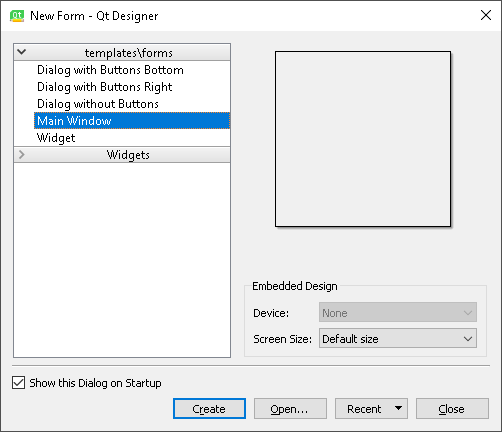
\includegraphics[scale=0.8]{imagenes/qtdesigner/qt_new_file.PNG}
    \caption{Ventana de creaci\'on de formas}
    \label{fig:qt_new_file}
\end{figure}

\subsection{BonusTrack: ¿Qu\'e cosas copadas tiene PyQt?}

\subsubsection{Ventanas de di\'alogo para reutilizar}
\label{dialogs_utiles}

Existen algunos di\'alogos ya creados por el framework de Qt para que reutilicemos,
como el \textbf{QFileDialog}, \textbf{QMessageBox}, \textbf{QColorDialog}, \textbf{QInputDialog}, \textbf{QProgressDialog},
entre otros... y su utilizaci\'on es muy sencilla. Observar en la Fig. \ref{fig:qt_dialog_examples}.

Se los puede utilizar configurandolos con el constructor, instanci\'andolos y luego llamando a alguno de sus m\'etodos para hacerlos
visibles y luego recuperar los datos que obtuvieron. Por otro lado, se pueden ejecutar desde alguno de sus m\'etodos est\'aticos.

\begin{figure}[H]
    \centering
    \begin{tabular}{c c}
        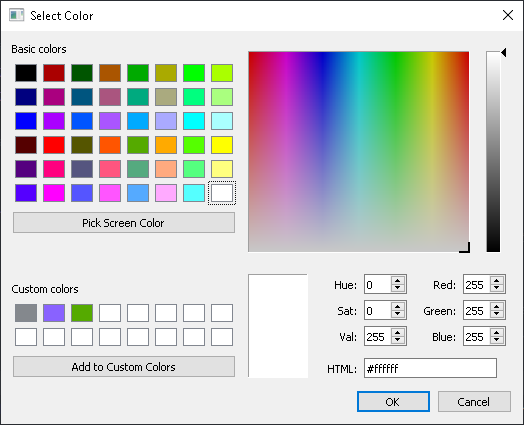
\includegraphics[scale=0.4]{imagenes/qtdesigner/qt_color_dialog.PNG} &
        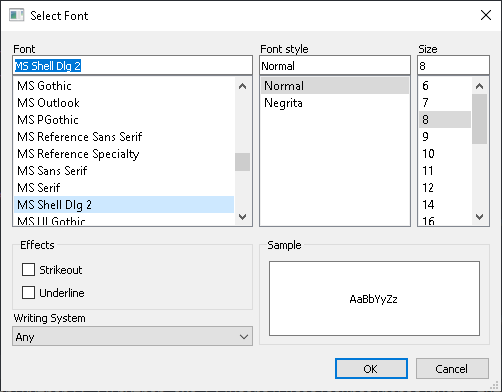
\includegraphics[scale=0.5]{imagenes/qtdesigner/qt_font_dialog.PNG} \\
        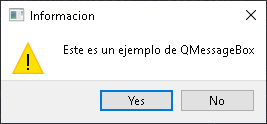
\includegraphics[scale=0.6]{imagenes/qtdesigner/qt_message_dialog.PNG} &
        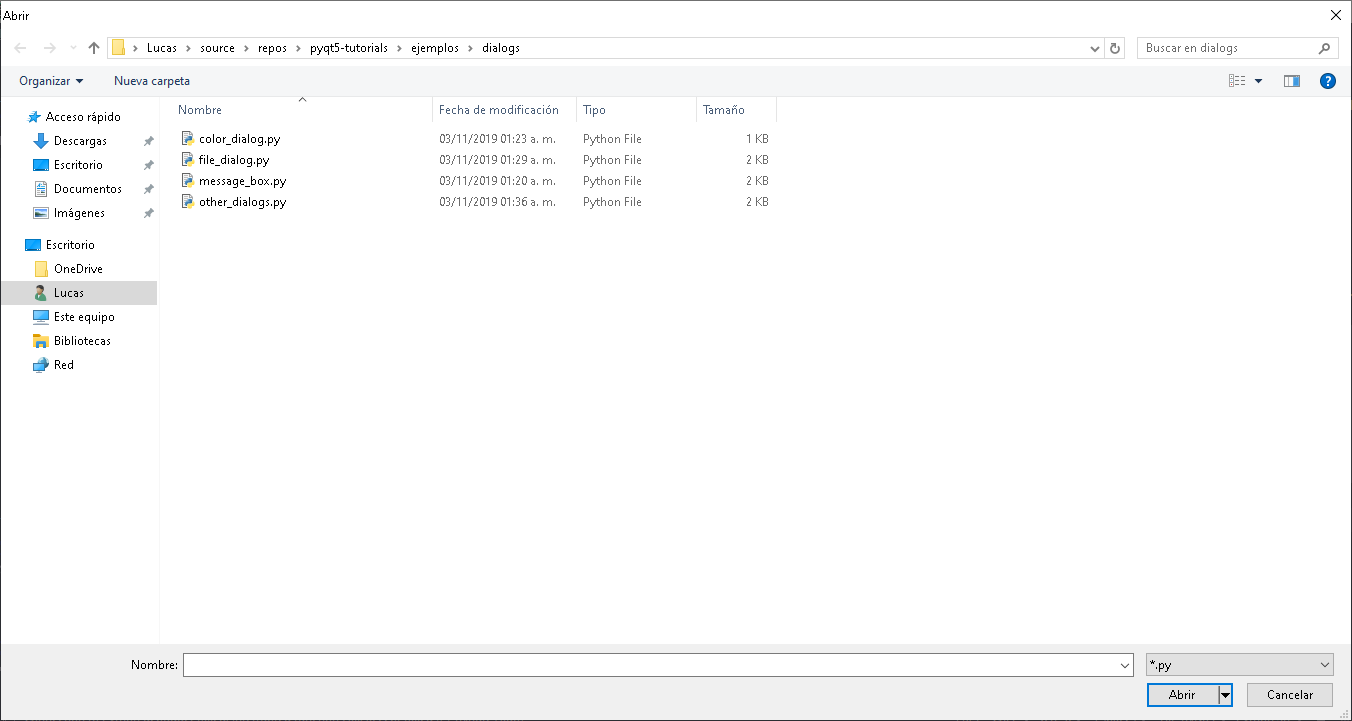
\includegraphics[scale=0.2]{imagenes/qtdesigner/qt_file_dialog.PNG} 
    \end{tabular}
    \caption{Ejemplos de QColorDialog, QFileDialog, QFontDialog y QMessageBox}
    \label{fig:qt_dialog_examples}
\end{figure}

